
\begin{figure}
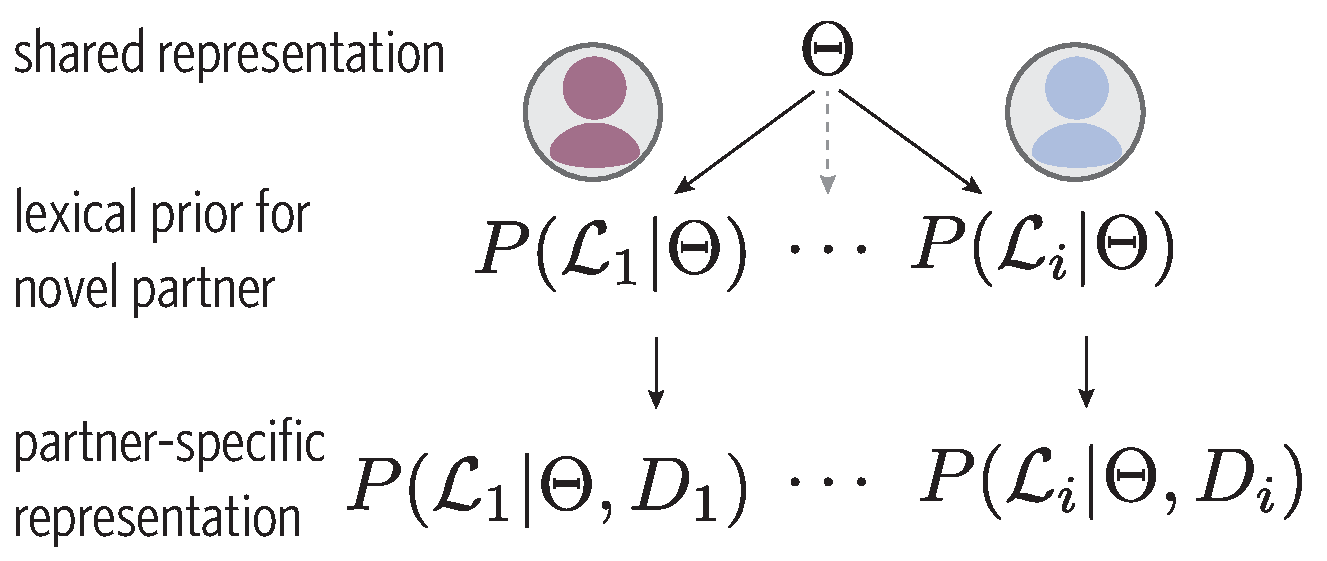
\includegraphics[scale=0.3]{./figures/task1_model.pdf}
\caption{Schematic of hierarchical Bayesian model.}
\label{fig:model_schematic}
\end{figure}

\subsection{Hierarchical inference: generalizing to new partners}

In this section, we provide an explicit computational account of the cognitive mechanisms supporting the balance between community-level stability and partner-specific flexibility.
Specifically, we show how the dyadic convention formation model of \cite{HawkinsetAl2017} can be extended with a principled mechanism for generalization across multiple partners.
This model begins with the idea that knowledge about linguistic meaning can be represented probabilistically: agents have uncertainty about the form-meaning mappings their current partner is using \cite{Bergen2016}. 
In our hierarchical model, this uncertainty is represented by a multi-level prior. 

At the highest level of the hierarchy is *community-level* uncertainty $P(\Theta)$, where $\Theta$ represents an abstract "overhypothesis" about the overall distribution of possible partners. 
$\Theta$ then parameterizes the agent's *partner-specific* uncertainty $P(\phi_{k} | \Theta)$, where $\phi_k$ represents the specific system of meaning used by partner $k$ (see Fig. \ref{fig:task1model}). 
Given observations $D_k$ from interactions with partner $k$, the agent updates their beliefs about the latent system of meaning using Bayes rule:
\begin{equation}
\begin{array}{rcl}
P(\phi_k, \Theta | D_k)  & \propto &  P(D_k | \phi_k, \Theta) P(\phi_k, \Theta) \\
                           & =   & P(D_k | \phi_k) P(\phi_k | \Theta) P(\Theta)
\end{array}
\end{equation}
This joint inference decomposes the learning problem into two terms, a prior term $P(\phi_k | \Theta)P(\Theta)$ and a likelihood term $P(D_k | \phi_k)$.
The prior captures the idea that different partners may share aspects of meaning in common.
In the absence of strong evidence that partner-specific language use departs from this common structure, the agent ought to regularize toward background knowledge of the population's conventions.
The likelihood represents predictions about how a partner using a particular system of meaning will use language.

This joint posterior over meanings has two consequences for convention formation.
First, it allows agents to maintain partner-specific expectations $\phi_k$ by marginalizing over community-level uncertainty:
\begin{equation}
P(\phi_k | D_k) = \int_{\Theta}P(D_k | \phi_k) P(\phi_k | \Theta) P(\Theta)  d\Theta
\end{equation}
Second, the hierarchical structure provides an inductive pathway for data to inform beliefs about community-wide conventions.
Agents update their beliefs about $\Theta$ by marginalizing over data accumulated from different partners:
\begin{equation}
P(\Theta | D) = P(\Theta) \int_{\phi} P(D_k | \phi_k) P(\phi_k | \Theta) d\phi
\end{equation}
where $D = \bigcup_{k=1}^N D_k$, $\phi = \phi_1 \times \dots \times \phi_N$, and $N$ is the number of partners previous encountered. 

After multiple partners are inferred to have a similar system of meaning, beliefs about $\Theta$ shift to represent this abstracted knowledge: it becomes more likely that a novel partner will share it as well.
This transfer is sometimes referred to as "sharing of strength" or "partial pooling" because pooled data is smoothly integrated with domain-specific knowledge.
